\begin{solution}
\begin{center}
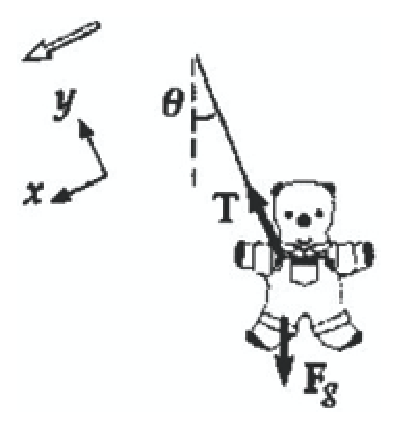
\includegraphics [scale=0.3]{./latex/eps/1_5_7_image_2.eps}
\end{center}
Dengan memilih arah sumbu x yaitu searah dengan bidang miring. Maka percepatan sumbu x menjadi
\begin{eqnarray*}
v_{f}&=&v_{i}+at \\
30 &=&0 + a(6) \\
a&=&5.0 \quad \textrm{$\frac{m}{s^{2}}$}
\end{eqnarray*}
Gaya-gaya untuk masing-masing komponen yaitu:
\begin{eqnarray*}
\Sigma F_{x}=ma_{x} \quad mg\sin\theta=m(5.0 m/s^{2}) \quad \textrm{maka} \quad \theta=30,7^{0} \\
\Sigma F_{y}=ma_{y} \quad -mg\cos\theta+T=0 \quad \textrm{maka} \quad T=0.843 \textrm{ N}
\end{eqnarray*}
\end{solution}
